\renewcommand{\columnseprule}{1.5pt}
\begin{multicols*}{2}
\noindent
\rule[0.5\baselineskip]{0.5\textwidth}{1pt}

\noindent
\subsection{Another Definition of Parabolas}
\noindent
1. In the past, you should've learned three forms of parabola equations.
Write the \textbf{standard form} of a parabola, the function
$f(x)$.  

\vspace{2cm}
\noindent
2. What is $f(0)$ and what does it represent on the graph?

\vspace{2cm}
\noindent
3. What is $a$?  Describe how various ranges of $a$ effect the graph.

\vspace{3cm}
\noindent
4. Hopefully, recall from memory what \textbf{vertex} form of a parabola
is.  If you must, you may search for the answer from a resource at hand.
Write a function $g(x)$ for a parabola with its vertex at $(h,k)$.

\vspace{3cm}
\noindent
5.  What if, instead, $x$ where a function of $y$?  What would vertex form
look like then?

\vspace{2cm}
\noindent
6. The remaining problems refer to the parabola shown here.
\begin{enumerate}
\item It has something called a \textbf{focus} at the point (6,0).
\item Its vertex is at the point (7,0).
\item It has something called a \textbf{directrix}, the line $x=8$.
\end{enumerate}
A point is shown on the parabola where $x=3$.  Its distance from the
directrix is $d_2$, and its distance from the focus is $d_1$.  Measure
these distances and show that $d_1 = d_2$.
 
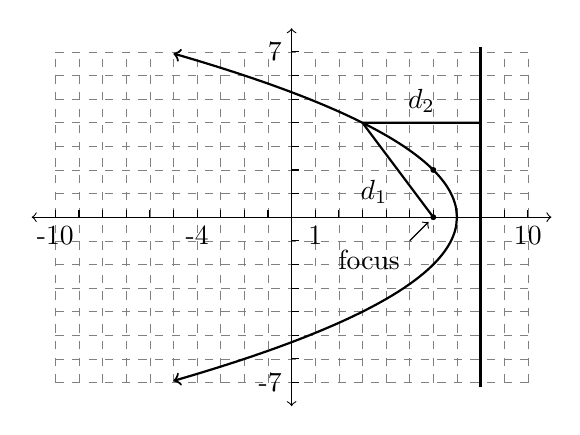
\begin{tikzpicture}[scale=0.3]
	\draw[dashed,gray,very thin] (-10,-7) grid (10,7);
	\draw [<->] (-11,0) -- (-10,0) node[anchor=north]{-10} 
		-- (-4,0) node[anchor=north]{-4} 
		-- (1,0) node[anchor=north]{1}
		-- (10,0) node[anchor=north]{10}
		-- (11,0);
	\draw [<->] (0,-8) -- (0,-7) node[anchor=east]{-7}
		-- (0,7) node[anchor=east]{7}
		-- (0,8);
	\draw [fill] (6,2) circle (0.1);
	\draw [thick, -] (6,0) 
		-- (4.5,2) node[anchor=north east] {$d_1$}
		-- (3,4) 
		-- (5.5,4) node[anchor=south] {$d_2$}
		-- (8,4);
	\foreach \i in {-10,-9,...,10} {
		\draw (\i,0) -- (\i,0.3);
    	}
	\foreach \i in {-7,-6,...,7} {
		\draw (0,\i) -- (0.3,\i);
	}
	\draw[domain=-5:7,<-,samples=400,thick] plot (\x,{sqrt(28-4*\x)});
	\draw[domain=-5:7,<-,samples=400, thick] plot (\x,{-1*sqrt(28-4*\x)});
	\draw[thick] (8,-7.2) -- (8,7.2);
	\draw[fill] (6,0)  circle (0.1);
	\draw[<-] (5.8,-0.2) -- (5,-1) node[anchor=north east] {focus};
\end{tikzpicture}

\noindent
7. Measure or calculate the focal distance and horizontal distance to the
directrix for $x=\{6,0,-4,7\}$.  Show that each time, $d_1=d_2$.

\vspace{3cm}
\noindent.

8. Pick a point on the parabola and call it $(x,y)$.  Using the distance
formula, calculate the focal distance and the directrix distance, and
set them equal to each other.  Eliminate the radical and simplify.

\vspace{3cm}
\noindent
9. Solve you equation for $y$ (using the $\pm$ symbol).  Enter these
two equations into your TI-8* and confirm they are the same as the
given graph.

\vspace{0.5cm}
\noindent
10.  Can we calculate the derivative of a function like this?  What would
such an equation look like and mean?

\vspace{2cm}
\noindent
11.  In your own words, describe what you think the point of this
problem set is.
\end{multicols*}
